\documentclass[a4paper]{article}

\usepackage[T1]{fontenc}
\usepackage{textcomp}
\usepackage{amsthm}
\usepackage{amsmath, amssymb}
\usepackage{enumitem}
\usepackage{import}
\usepackage{xifthen}
\usepackage{transparent}
\usepackage[affil-it]{authblk}

\usepackage{listings}
\usepackage{color}
\usepackage{float}
\usepackage{pgfplots}

\usepgfplotslibrary{polar}
\usepgflibrary{shapes.geometric}

% Settings
\pgfplotsset{my style/.append style={axis x line=middle, axis y line=middle, xlabel={$x$}, ylabel={$y$}, axis equal}}
\definecolor{dkgreen}{rgb}{0,0.6,0}
\definecolor{gray}{rgb}{0.5,0.5,0.5}
\definecolor{mauve}{rgb}{0.58,0,0.82}

\lstset{frame=tb,
  language=Python,
  aboveskip=3mm,
  belowskip=3mm,
  showstringspaces=false,
  columns=flexible,
  basicstyle={\small\ttfamily},
  numbers=none,
  numberstyle=\tiny\color{gray},
  keywordstyle=\color{blue},
  commentstyle=\color{dkgreen},
  stringstyle=\color{mauve},
  breaklines=true,
  breakatwhitespace=true,
  tabsize=3
}
% title
\title{COMP 361: Elementary Numerical Methods\\
Term test 2 Graphs}

\author{Duc Nguyen}
 \affil{Gina Cody School of Computer Science and Software Engineering \\
    Concordia University, Montreal, QC, Canada}
\date{Winter 2020}

\begin{document}
\maketitle

\newpage
\section{Graph of the iteration for problem 7}
% Graph of the iteration Problem 8
\begin{figure}[H]
\centering
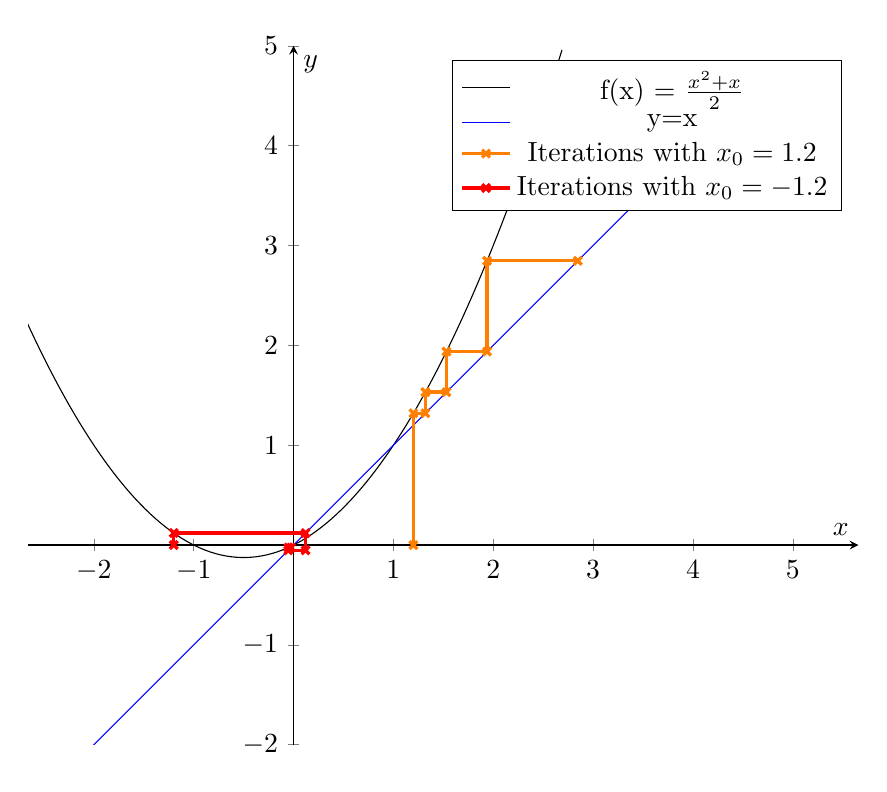
\begin{tikzpicture}
   \begin{axis}[my style,restrict y to domain=-5:5,width=\linewidth, xmin=-2, xmax=5,ymin=-2,ymax=5]
       \addplot[samples=200]{(x^2+x)/2};
       \addlegendentry{f(x) = $\frac{x^{2} + x}{2}$}
      \addplot[domain=-4:4,color=blue]{x};
      \addlegendentry{y=x}
      \addplot[mark=x,color=orange,very thick] coordinates {
          (1.2,0) (1.2, 33/25) (33/25, 33/25) (33/25, 957/625) (957/625, 957/625) (957/625, 1.93789)
          (1.93789, 1.93789) (1.93789, 2.846645) (2.846645, 2.846645)
      };
      \addlegendentry{Iterations with $x_{0} = 1.2$}

      \addplot[mark=x,color=red,very thick] coordinates {
          (-1.2, 0)(-1.2, 3/25)(3/25, 3/25)(3/25, -33/625)(-33/625, -33/625) (-33/625, -0.025006)(-0.025006, -0.025006)
      };
      \addlegendentry{Iterations with $x_{0} = -1.2$}
   \end{axis}
\end{tikzpicture}
\caption{Fixed point iteration diagram}
\end{figure}

\newpage
\section{Graph of the iteration for problem 8}
% Graph of the iteration Problem 8
\begin{figure}[H]
\centering
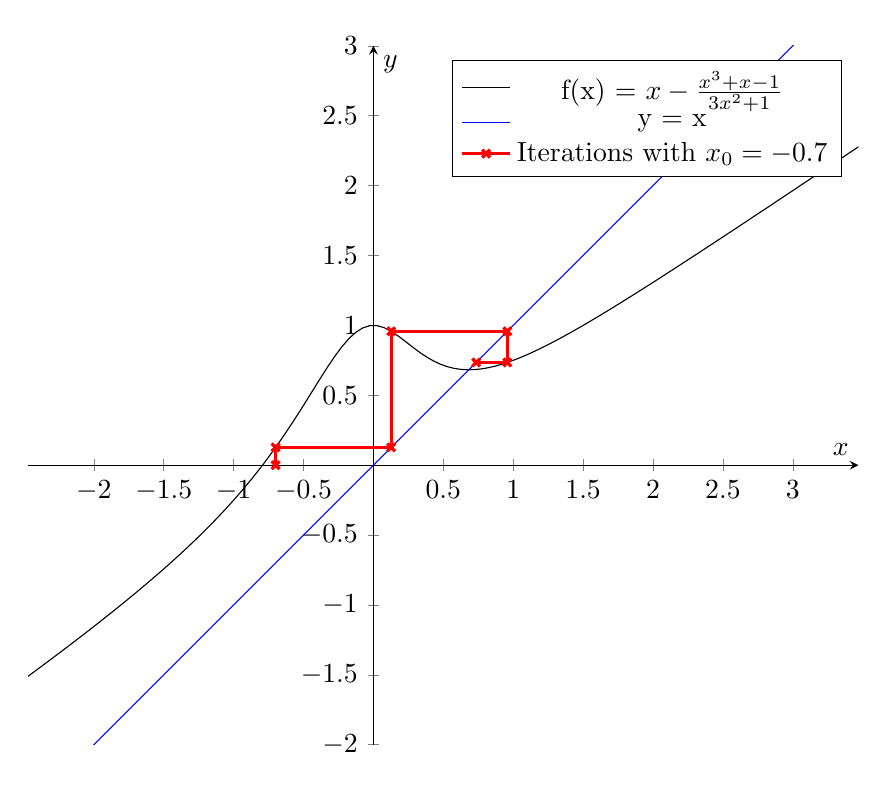
\begin{tikzpicture}
   \begin{axis}[my style,restrict y to domain=-5:5,width=\linewidth, xmin=-2, xmax=3,ymin=-2,ymax=3]
       \addplot[samples=200]{x-(x^3+x-1)/(3*x^2+1)};
       \addlegendentry{f(x) = $x - \frac{x^{3} + x - 1}{3x^{2} + 1} $}
      \addplot[domain=-4:4,color=blue]{x};
      \addlegendentry{y = x}
      \addplot[mark=x,color=red,very thick] coordinates {
          (-0.7,0) (-0.7, 0.127126) (0.127126, 0.127126) (0.127126, 0.957678) (0.957678, 0.957678) (0.957678, 0.7348278) (0.7348278, 0.7348278) 
      };
      \addlegendentry{Iterations with $x_0 = -0.7$}
   \end{axis}
\end{tikzpicture}
\caption{Fixed point iteration diagram}
\end{figure}
\newpage

\end{document}
